\section{Scheduling}

\paragraph{Motivation}
\begin{items}
  \item \( K \) jobs ready to run, \( K > N \geq 1 \) CPUs available
  \item \textbf{Scheduling Problem}: \\*
    - Which jobs should kernel assign to which CPUs? \\*
    - When should it make decision?
\end{items}

\paragraph{Dispatcher}
\begin{items}
  \item \textbf{Dispatcher}: performs actual process switch \\*
    - mechanism \\*
    - save/restore process context \\*
    - switch to user mode
  \item \textbf{Scheduler}: selects next process to run based on \emph{policy}
\end{items}

\paragraph{Voluntary Yielding vs. Preemption}
\begin{items}
  \item kernel responsible for CPU switch
  \item kernel doesn't always run \( \to \) can only dispatch different process when invoked
  \item \textbf{cooperative multitasking}: running process performs \emph{yield} syscall \( \to \) kernel switches process
  \item \textbf{preemptive scheduling}: \\*
    - kernel invoked in certain time intervals \\*
    - kernel makes scheduling decisions after every time-slice
\end{items}
\begin{figure}[H]\centering\label{ProcessSwitching}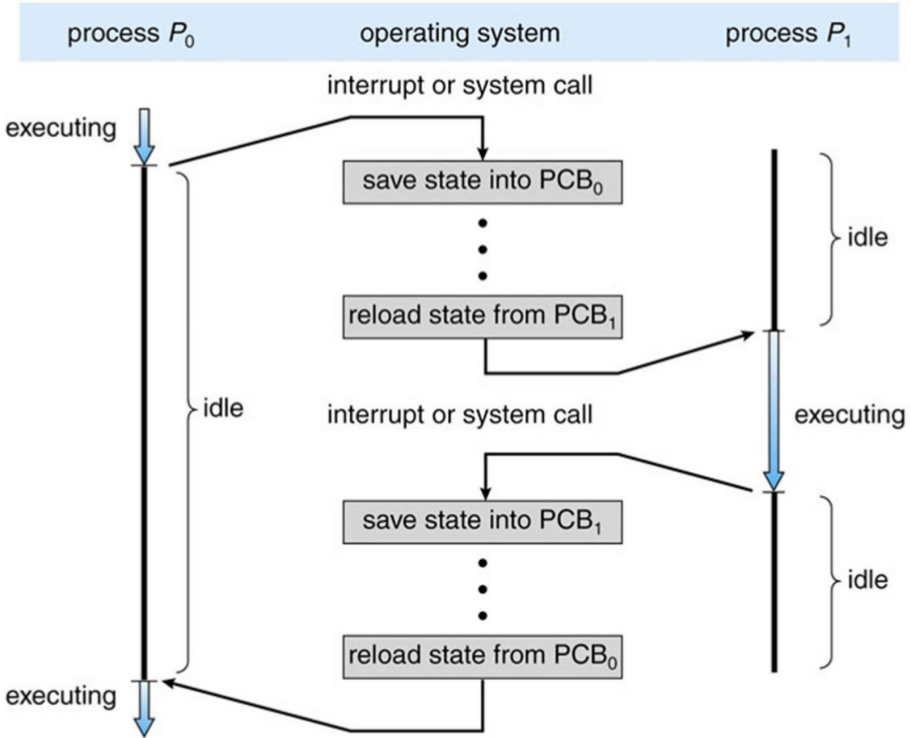
\includegraphics[width=0.33\textwidth]{ProcessSwitching}\end{figure}

\paragraph{Scheduling --- Process States}
\begin{items}
  \item \textbf{new}: process was created but did not run yet
  \item \textbf{running}: instructions are currently being executed
  \item \textbf{waiting}: process is waiting for some event
  \item \textbf{ready}: process is waiting to by assigned a processor
  \item \textbf{terminated}: process has finished execution
\end{items}

\paragraph{Scheduling --- long-term vs. short-term}
\begin{items}
  \item \textbf{Short-term scheduler} (CPU Scheduler, focused on in this lecture): \\*
    - selects process to run next, allocates CPU \\*
    - invoked frequently (ms) \( \leadsto \) must be fast
  \item \textbf{Long-term scheduler} (job scheduler): \\*
    - selects process to be brought into ready queue \\*
    - invoked very infrequently (s, m) \( \leadsto \) can be slow \\*
    - controls degree of \emph{multiprogramming}
\end{items}

\paragraph{Scheduling queues}
\begin{items}
  \item \textbf{job queue}: set of all processes in system
  \item \textbf{ready queue}: process in main memory, ready or waiting
  \item \textbf{device queue}: processes waiting for I/O device
\end{items}

\paragraph{Scheduling Policies --- Categories}
\begin{items}
  \item \textbf{batch scheduling}: \\*
    - still widespread in business (payroll, inventory,\dots) \\*
    - no users waiting for quick response \\*
    - non-preemptive algorithms acceptable \( \to \) less switches \( \to \) less overhead
  \item \textbf{interactive scheduling}: \\*
    - need to optimize for response time \\*
    - preemption essential to keep processes from hogging CPU
  \item \textbf{real-time scheduling}: \\*
    - guarantee job completion within time constraints \\*
    - need to be able to plan when which process runs + how long \\*
    - preemption not always needed
\end{items}

\paragraph{Scheduling Policies --- Goals}
\begin{items}
  \item \textbf{General}: \\*
    - \emph{fairness}: give each process fair share of CPU \\*
    - \emph{balance}: keep all parts of system busy
  \item \textbf{batch scheduling}: \\*
    - \emph{throughput}: number of processes that complete per time unit \\*
    - \emph{turnaround time}: time from job submission to job completion \\*
    - \emph{CPU utilization}: keep CPU as busy as possible
  \item \textbf{interactive scheduling}: \\*
    - \emph{waiting time}: reduce time a process waits in waiting queue \\*
    - \emph{response time}: time from request to first response
  \item \textbf{real-time scheduling}: \\*
    - \emph{meeting deadlines}: finishing jobs in time \\*
    - \emph{predictability}: minimize jitter
\end{items}

\paragraph{Scheduling Policies --- first come first served}
\begin{items}
  \item intuitively clear
  \item \textbf{Example}: 3 processes arrive at time 0 in the order \( P_1, P_2, P_3 \)
    \begin{center}
      \begin{tabular}{|c|c|c|}
        \textbf{Process} & \textbf{Burst time} & \textbf{Turnaround time} \\
        \hline
        \( P_1 \) & 24 & 24 \\
        \( P_2 \) & 3 & 27 \\
        \( P_3 \) & 3 & 30
      \end{tabular}
    \end{center}
  \item \( \leadsto \) average turnaround time 27 \( \to \) \emph{can we do better?}
  \item \textbf{Conclusion}: if processes would arrive in order \( P_2 \), \( P_3 \), \( P_1 \), average turnaround time would be 13 \\*
    \( \leadsto \) \emph{good scheduling can reduce turnaround time}
\end{items}

\paragraph{Scheduling Policies --- shortest job first}
\begin{items}
  \item \textbf{Benefits}: optimal average turnaround/waiting/response time
  \item \textbf{Challenge}: cannot know job lengths in advance
  \item \textbf{Solution}: predict length of next CPU burst for each process \\*
    \( \leadsto \) schedule process with shortest burst next
  \item \textbf{Burst Estimation}: \emph{exponential averaging} \\*
    - \( \tau_{n+1} = \alpha t_n + (1-\alpha)\tau_n \) \\* \phantom{-} (\( t_n \): actual length of \( n \)-th CPU burst, \( \tau_{n+1} \): predicted length of next CPU burst, \( 0 \leq \alpha \leq 1 \))
\end{items}

\paragraph{Process Behavior --- CPU bursts}
\begin{items}
  \item CPU bursts exists because processes wait for I/O
  \item \textbf{CPU-bound processes}: spends more time doing computations \\*
    \( \leadsto \) few very long CPU bursts
  \item \textbf{I/O-bound processes}: spends more time doing I/O \\*
    \( \leadsto \) many short CPU bursts
\end{items}

\paragraph{Scheduling Policies --- preemptive shortest-job-first}
\begin{items}
  \item SJF optimizes waiting/response time \\*
    \( \leadsto \) what about throughput?
  \item \textbf{Problem}: CPU-bound jobs hold CPU until exit or I/O \( \to \) \emph{poor I/O utilization}
  \item \textbf{Idea}: SJF, but preempt periodically to make new scheduling decision \\*
    - each time slice: schedule job with shortest remaining time next \\*
    - alternatively: schedule job with shortest next CPU burst
\end{items}

\paragraph{Scheduling Policies --- round robin}
\begin{items}
  \item \textbf{Problem}: batch schedulers suffer from starvation and don't provide fairness
  \item \textbf{Idea}: each process runs for small CPU time unit \\*
    - \emph{time quantum}/\emph{time slice} length: usually 10-100ms \\*
    - preempt processes that have not blocked by end of time slice \\*
    - append current thread to end of run queue, run next thread
  \item \textbf{Caution}: time slice length needs to balance interactivity and overhead! \\*
    \( \to \) if time slice length in the area of dispatch time, 50\% of CPU time wasted for process switching
\end{items}

\paragraph{Scheduling Policies --- virtual round robin}
\begin{items}
  \item \textbf{Problem}: RR is unfair for I/O-bound jobs: they block before using up time quantum
  \item \textbf{Idea}: put jobs that didn't use up their quantum in additional queue \\*
    - store share of unused time-slice \\*
    - give those jobs additional queue priority \\*
    - put them back into normal queue afterwards
\end{items}

\paragraph{Scheduling Policies --- (strict) priority scheduling}
\begin{items}
  \item \textbf{Problem}: not all jobs are equally important \\*
    \( \leadsto \) different priorities (e.g., 4)
  \item \textbf{Solution}: associate priority number with each process \\*
    - RR for each priority \\*
    - \emph{aging}: old low priority processes get executed before new higher priority processes
\end{items}

\paragraph{Scheduling Policies --- multi-level feedback queue}
\begin{items}
  \item \textbf{Problem}: context switching expensive \\*
    \( \leadsto \) trade-off between interactivity and overhead?
  \item \textbf{Goals}: \\*
    - higher priority for I/O jobs (usually don't use up quantum) \\*
    - low priority for CPU jobs (rather run them longer)
  \item \textbf{Idea}: different queues with different priorities and time slice lengths \\*
    - schedule queues with (static) priority scheduling \\*
    - double time slice length in each next-lower priority \\*
    - process to higher priority when they don't use up quantum repetitively \\*
    - process to lower priority when they use up quantum repetitively
\end{items}

\paragraph{Scheduling Principles --- priority donation}
\begin{items}
  \item \textbf{Problem}: Process B (higher priority) waits for process A (lower priority) \\*
    \( \leadsto \) B has now effectively lower priority
  \item \textbf{Solution}: \emph{priority donation} \\*
    - give A priority of B as long as B waits for A \\*
    - if C, D, E wait for B \( \to \) A gets highest priority of B, C, D, E
\end{items}

\paragraph{Scheduling Policies --- lottery scheduling}
\begin{items}
  \item issue number of lottery tickets to processes (amount depending on priority)
  \item amount of tickets controls average proportion of CPU for each process
  \item \textbf{Scheduling}: scheduler draws random number \( N \), process with \( N \)-th ticket is executed
  \item processes can transfer tickets to other processes if they wait for them
\end{items}

\begin{summary}
  \begin{items}
    \item \textbf{phases}: processes have phases of communication and waiting for I/O \\*
      $ \to $ appropriate switching between processes increases computing system utilization
    \item \textbf{goal-based}: scheduler decides what appropriate means based on goals \\*
      $ - $ \emph{long-term scheduler}: degree of multiprogramming \\*
      $ - $ \emph{short-term scheduler}: which process to run next
    \item \textbf{dispatching}: only happens when OS is invoked \\*
      $ - $ \emph{cooperative scheduling}: currently running thread yields (syscall) \\*
      $ - $ \emph{preemptive scheduling}: OS is called periodically to switch threads
  \end{items}
\end{summary}